Модели статических и динамических систем, построение, использование и анализ которых базируется на положениях теории нечётких множеств, называют нечёткими моделями~\cite{Borisov_Fedulov}. Многие исследователи отмечают тот факт, что нечёткие модели могут рассматриваться как обобщение интервальных, которые, в свою очередь, обобщают известные чёткие модели. К примеру, рассмотрим некоторую функцию $y=f \left(x \right)$, которую, с точки зрения дискретной математики, можно представить как отношение на декартовом произведении $X \times Y$. Вне зависимости от типа модели, вычисление выходного значения $y$ для заданного значения входного параметра $x$ происходит в три этапа~\cite{Borisov_Fedulov}:
\begin{itemize}
	\item задание значения входной переменной $x \in X$;
	\item нахождение пересечения $x$ с отношением $f$;
	\item проецирование пересечения $x$ и $f$ на $Y$.
\end{itemize}

Однако результаты во всех случаях различны по своему роду. На рисунке~\ref{fig:functypes-restypes} приведены результаты вычислений для чёткой, интервальной и нечёткой функций при различных видах аргументов.

\begin{figure}[pH]
  \centering
  \begin{subfigure}[t]{0.4\textwidth}
    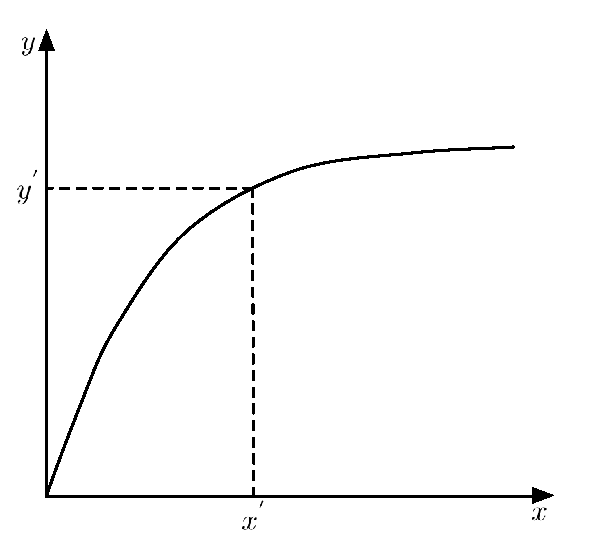
\includegraphics[width=\textwidth]{crisp-f-crisp-xy}
    \caption{Чёткая функция, чёткий аргумент}
  \end{subfigure}
  \quad
  \begin{subfigure}[t]{0.4\textwidth}
    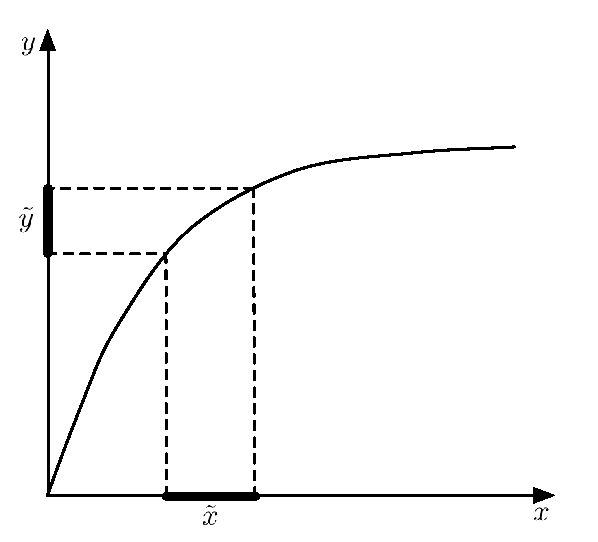
\includegraphics[width=\textwidth]{crisp-f-fuzzy-xy}
    \caption{Чёткая функция, нечёткий/интервальный аргумент}
  \end{subfigure}
  
  \begin{subfigure}[h]{0.4\textwidth}
    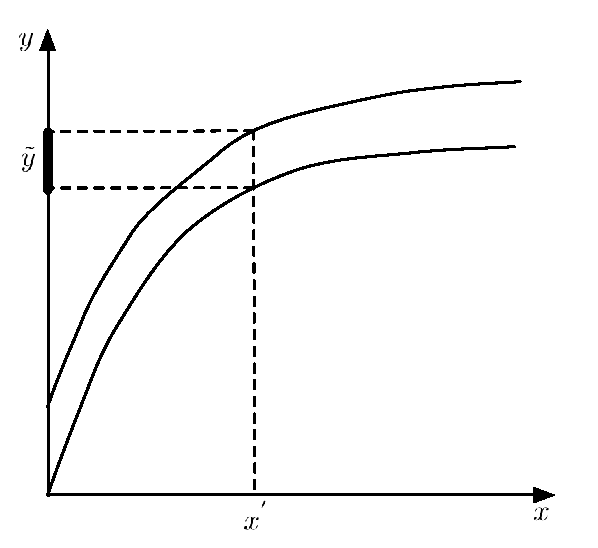
\includegraphics[width=\textwidth]{interval-f-crisp-xy}
    \caption{Интервальная функция, чёткий аргумент}
  \end{subfigure}
  \quad
  \begin{subfigure}[h]{0.4\textwidth}
    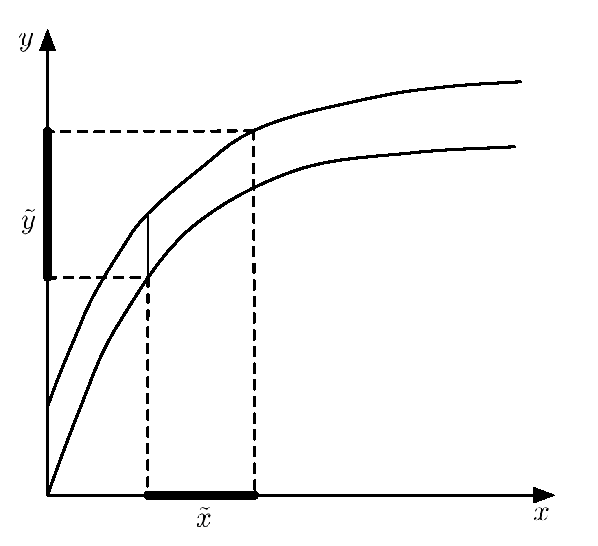
\includegraphics[width=\textwidth]{interval-f-fuzzy-xy}
    \caption{Интервальная функция, интервальный/нечёткий аргумент}
  \end{subfigure}
  
  \begin{subfigure}[b]{0.4\textwidth}
    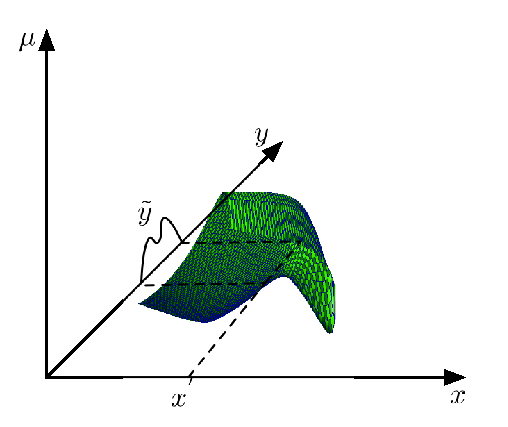
\includegraphics[width=\textwidth]{fuzzy-f-crisp-xy}
    \caption{Нечёткая функция, чёткий аргумент}
  \end{subfigure}
  \quad
  \begin{subfigure}[b]{0.4\textwidth}
    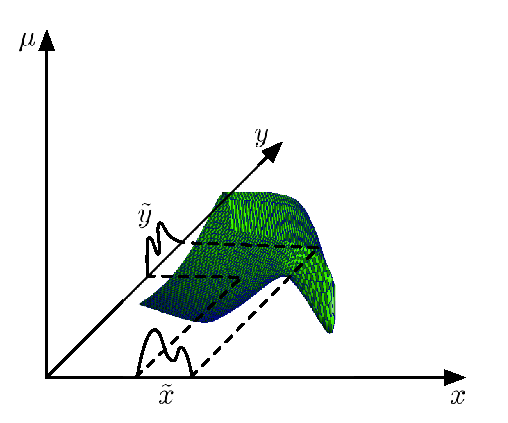
\includegraphics[width=\textwidth]{fuzzy-f-fuzzy-xy}
    \caption{Нечёткая функция, интервальный/нечёткий аргумент}
  \end{subfigure}
  \caption{Результаты вычислений для чётких, интервальных и нечётких функций при чётких и нечётких параметрах}
  \label{fig:functypes-restypes}
\end{figure}

На основании этого примера и категорий неопределённости, выделенных в~\cite{Yarushkina}, можно выделить взаимосвязи между описаниями и переменными чётких и нечётких моделей, а также математические методы, которые применимы для описания моделей. Выделенные взаимосвязи изображены в таблице~\ref{t:fuzzy-modeling-approaches}.
\begin{table}[h!]
\caption{Взаимосвязи между описаниями и переменными чётких и нечётких моделей}
\label{t:fuzzy-modeling-approaches}
\begin{center}
\begin{tabularx}{\textwidth}{|p{0.15\linewidth}|p{0.15\linewidth}|p{0.15\linewidth}|X|}
	\hline
		\centering \textit{Описание модели} & \centering \textit{Входные данные} & \centering \textit{Выходные данные} & \centering \textit{Математические методы} \tabularnewline	\hline
	\hline
		Чёткое & Чёткие & Чёткие & Функциональный анализ, линейная алгебра и т.д. \tabularnewline
	\hline
		Чёткое & Нечёткие & Нечёткие & Принцип обобщения Заде \tabularnewline
	\hline
		Чёткое & Нечёткие & Чёткие & Нечёткие модели и вычисления \tabularnewline
	\hline
		Нечёткое & Чёткие/\allowbreak Нечёткие & Нечёткое & Нечёткие модели и вычисления \tabularnewline
  \hline
\end{tabularx}
\end{center}
\end{table}

Очевидно, что нечёткое моделирование не подменяет собой другие методологии моделирования сложных систем, в которых существенные зависимости выражены настолько хорошо, что они могут быть выражены в числах или символах, получающих в итоге численные оценки~\cite{Borisov_Fedulov}. Нечёткие модели скорее представляют необходимый инструмент для исследования как отдельных аспектов, так и системы в целом на различных этапах её анализа в случае доминирования качественных элементов над количественными. Об этом же говорится и в~\cite{Kaufmann, Borisov_Alexeev_Msk}~--- теория нечётких множеств не призвана конкурировать с теорией вероятности и статистическими методами, она заполняет пробел в области структуризованной неопределённости там, где нельзя корректно применять статистику и вероятности ввиду неизвестности распределения величин или малого размера статистической выборки.

В~\cite{Borisov_Fedulov} предложена оригинальная классификация подходов к созданию нечётких моделей в~зависимости от~того, в~какой момент моделирования используется теория нечётких множеств, а~также соответствующие ей сферы применения нечётких моделей. Рассмотрим данную классификацию подробнее: нечёткость может применяться
\begin{enumerate}
	\item при описании системы~--- речь идёт об информационной неопределённости~\cite{Pospelov, Borisov_Alexeev_Msk}. Система описывается моделями нечёткой логики: продукционными/реляционными/функциональными. Обычно такой подход применяется, когда имеются неполные или неопределённые знания об исследуемом объекте, а их дополнение является либо невозможным, либо нецелесообразным, либо значительная часть информации об объекте является качественной и не~выражается с~помощью известных математических зависимостей, но может быть описана системой предпочтений на~естественном языке в форме правил <<если-то>>;
	\item при задании параметров системы~--- в традиционной, чёткой модели системы используются нечёткие параметры (например, нечёткие коэффициенты обычных алгебраических или дифференциальных уравнений). Данный подход оправдывает себя в ситуации полной определённости модели, когда необходимо учесть присущую параметрам неопределённость, а традиционный вероятностный подход неприменим ввиду того, что неоднозначность параметров не является физической согласно классификации, используемой в~\cite{Borisov_Alexeev_Msk, Yarushkina}. В таких ситуациях приходится прибегать к~услугам экспертов, которые выражают своё мнение в виде качественных оценок, а принадлежность объектов задаётся с помощью лингвистических операторов («много», «мало», «около» и т.п.);
	\item нечёткость при~задании входов, выходов и состояний системы~--- в традиционной модели системы с чёткими или нечёткими параметрами могут применяться нечёткие переменные. Этот подход в основном применяется при идентификации динамических или нелинейных систем на основе их входных и выходных параметров~\cite{Fuller} и позволяет при наличии обучающей выборки аппроксимировать искомые функции или измеренные данные с наперёд заданной точностью;
	\item комбинированные модели~--- создаются на основе совмещения двух или более подходов.
\end{enumerate}

Если рассматривать описанную выше классификацию подходов к синтезу нечётких моделей через призму выбора, который являются неотъемлемой частью моделирования как целенаправленного процесса, и языков его описания, то можно заметить, как модель и используемый в ней язык выбора проецируются на~два основных раздела современной нечёткой математики~--- нечёткий логический вывод и мягкие вычисления. К настоящему моменту сложилось три основных языка описания выбора~--- язык функций выбора, язык бинарных отношений и критериальный язык~\cite{Choice_Languages}, которые позволяют говорить об одном и том же объекте или явлении с разной степенью общности. Два последних языка~--- язык бинарных отношений и критериальный язык~--- достаточно хорошо изучены и отражены в рамках теории нечётких множеств. Схематически взаимосвязи между сферами нечёткого моделирования и~языками выбора изображены на~рисунке~\ref{fig:choice-classes}.

\begin{figure}[t!]
  \centering{
    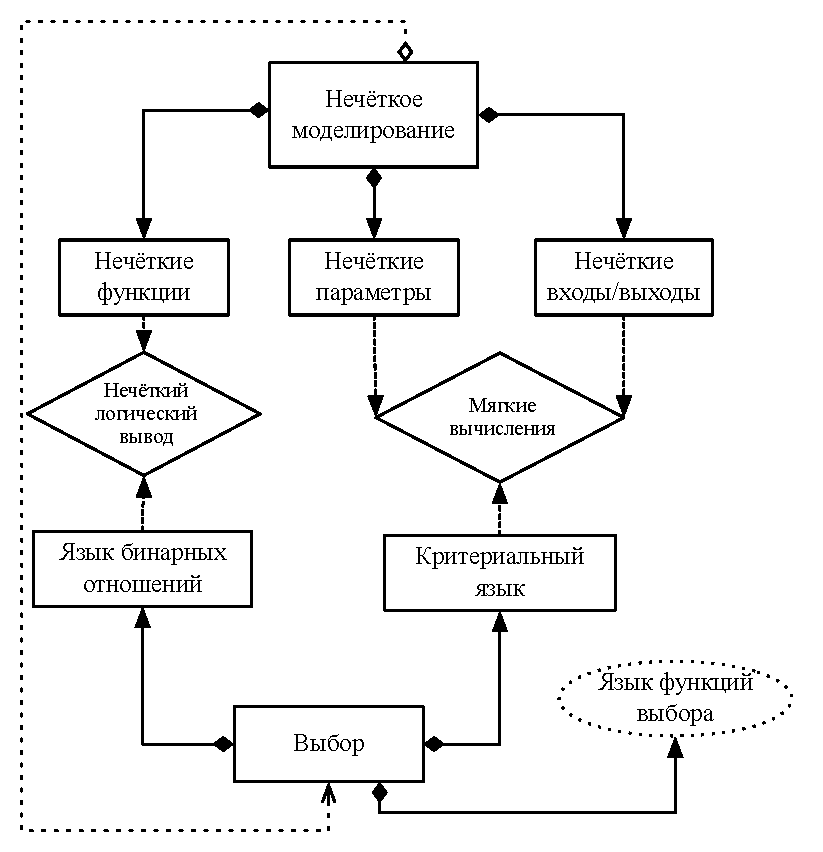
\includegraphics[width=0.7\textwidth]{choice-classification}
    \caption{Связь между языками описания выбора и нечётким моделированием}
    \label{fig:choice-classes}
  }
\end{figure}

Язык бинарных отношений является более общим и основывается на том факте, что в~реальности дать объективную оценку той или~иной альтернативе затруднительно или невозможно, однако, при~рассмотрении альтернатив в~паре, можно указать более или~менее предпочтительную. Основные предположения этого~языка выбора сводятся к~следующим:
\begin{itemize}
	\item отдельная альтернатива не~оценивается;
	\item для~каждой пары альтернатив некоторым образом можно установить, что~одна из~них предпочтительнее другой, либо они равноценны или несравнимы;
	\item отношение предпочтения внутри любой пары альтернатив не~зависит от~остальных альтернатив, предъявленных к~выбору.
\end{itemize}

Нечёткие модели первого типа, в которых нечёткость присутствует на этапе описания системы~\cite{Choice_Languages}, как раз используют язык бинарных отношений. В~нечёткой математике этот язык проецируется на нечёткий логический вывод и основанное на нём нечёткое управление. Основополагающими для логического вывода являются понятия нечёткого отношения, лингвистической переменной и нечёткой импликации, на которой основаны правила логического вывода.

\begin{mydef}
Лингвистической переменной называется переменная, значения которой представляют слова или суждения на естественном языке. С точки зрения нечёткой математики, это кортеж $\left\lbrace \beta, T, X, G, M \right\rbrace$, где $\beta$~--- название нечёткой переменной; $T$~--- базовое терм-множество лингвистической переменной, каждый элемент которого (терм) представляется как нечеткое множество на универсальном множестве $X$; $G$~--- cинтаксические правила, часто задаваемые в виде грамматики, для порождения названий термов; $M$~--- семантические правила, задающие функции принадлежности нечетких термов, порожденных синтаксическими правилами $G$ \cite{Uskov_Kuzmin, Uskov_Kruglov, Shtovba}.
\end{mydef}

\begin{mydef}
Нечёткая импликация является нечётким отношением $\tilde R \subseteq X \times Y$, простейшая форма которого выражается в~виде правила <<если-то>>~\cite{Pegat}
\begin{equation}
  IF \left( x = \tilde A \right) THEN \left( y = \tilde B\right),\ x \in X, y \in Y.
\end{equation}
Нечёткая импликация обозначается как $\tilde A \rightarrow \tilde B$ и, как любое другое нечёткое отношение, задаётся функцией принадлежности.
\end{mydef}
В~\cite{Pegat, Rutkovskaya} описаны несколько применяемых на практике операторов импликации, задаваемых различными функциями принадлежности (например, операторы Мамдани, Лукасевича, Ларсена, Гёделя, Ягера, Заде).

На основании нечётких переменных и правил импликации строятся модели нечёткого логического вывода и управления. Типовая модель включает в~себя четыре основных блока~\cite{Fuller}, изображённые на рисунке~\ref{fig:general-fuzzy-inference}~--- блок фаззификации, который сопоставляет чётким входным значениям нечёткие множества; блок нечёткого логического вывода, опирающийся на базу правил, хранящуюся в виде нечётких импликаций <<если-то>>; блок дефаззификации, который на основании результирующей функции принадлежности формирует чёткое выходное значение с помощью одного из методов дефаззификации (центра тяжести, первого/среднего/последнего максимума, центра сумм и др.)~\cite{Pegat, Uskov_Kuzmin, Uskov_Kruglov, Zak}. Наиболее популярными моделями являются нечёткие контроллеры Такаги-Сугено и~Мамдани, применяемые, в частности, в~качестве нечётких регуляторов в~промышленной и~бытовой электронике~\cite{Grinyaev_Computerra}.

\begin{figure}[h!]
  \centering{
    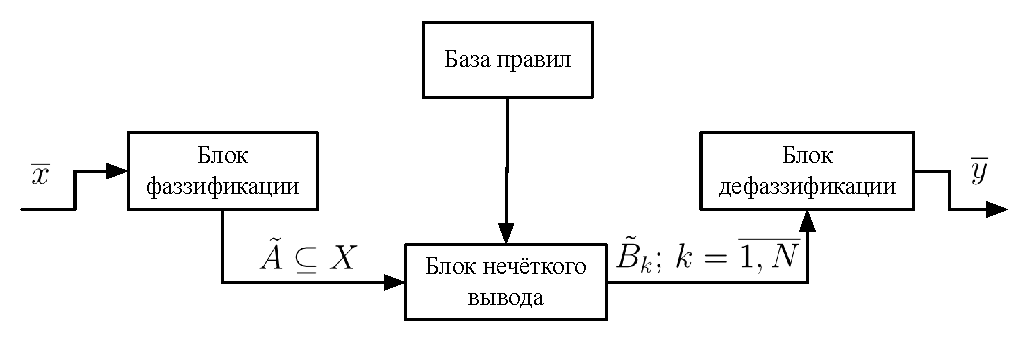
\includegraphics[width=\textwidth]{fuzzy-inference}
    \caption{Общая схема системы нечёткого управления}
    \label{fig:general-fuzzy-inference}
  }
\end{figure}

Достоинства и недостатки, а также рекомендации по применению нечёткого логического вывода и нечёткого управления хорошо описаны в~\cite{Bauer_Winkler, Grinyaev_Computerra}. Согласно~\cite{Bauer_Winkler, Pavlov_Sokolov}, использование моделей первого типа рекомендуется для моделирования очень сложных процессов, когда не существует простой математической модели, для нелинейных процессов высоких порядков и для~обработки лингвистически сформулированных экспертных знаний. Ещё одним преимуществом является наличие нескольких подходов к проверке моделей на устойчивость~\cite{Pegat, Uskov_Kruglov}. Эти же модели не рекомендуется применять, если приемлемый результат может быть получен с~помощью общей теории управления, либо существует формализованная и адекватная математическая модель, либо проблема не разрешима методами современной математики. Также модели нечёткого управления страдают от~<<проклятия размерности>>~--- с увеличением числа входов лавинообразно нарастает число необходимых правил для вывода~\cite{Pegat, Fuller}. Нечёткому логическому выводу и~управлению посвящено множество книг и~публикаций, однако подробное рассмотрение моделей первого вида выходит за~рамки данной диссертации.

Второй язык, более простой и~узкий, однако и~более изученный~--- критериальный. Он~основывается на~предположении, что~каждую отдельно взятую альтернативу возможно оценить конкретным числом, называемым значением критерия. Сравнение альтернатив в~таком случае сводится к~сравнению соответствующих~им числовых значений. Пусть $x\in X$ - некоторая альтернатива из~множества альтернатив $X$. Критерием будем называть функцию $q\left( x \right),\ x\in X$, обладающую тем~свойством, что~если альтернатива ${x_1}$ предпочтительнее ${x_2}$, то $q\left( x_1 \right)>q\left( x_2 \right)$ и~наоборот. Естественно считать, что наилучшей альтернативой ${{x}^{*}}$ считается~та, значение критерия которой максимально:
\begin{equation*}
  x^{*}=\arg \underset{i}{\mathop{\max }}\,\left\{ q\left( x_i \right) \right\}.
\end{equation*}
Задача отыскания $x^{*}$, достаточно простая по~постановке, часто оказывается весьма сложной в решении, поскольку зависит от характера множества $X$ и критерия $q\left( x \right)$. 

Нечёткие модели второго и третьего типа, в которых нечёткими являются либо их параметры, либо состояния и входные и выходные данные, описываются с помощью критериального языка. Этот язык в~нечёткой~математике соответствует т.\,н. <<мягким вычислениям>>~--- нечётким множествам, нечётким числам и определённым на них алгебрам. Как уже упоминалось ранее, описание с помощью нечётких множеств имеет существенные преимущества перед языком теории вероятностей в том случае, когда имеется лингвистическая неоднозначность в смысле полисемии~\cite{Borisov_Alexeev_Msk}, и~оценки получаются c помощью опроса экспертов. Известно, что люди в большинстве своём неправильно оценивают вероятности (особенно большие и малые), поэтому требовать от экспертов, коими обычно являются специалисты в конкретных предметных областях, а не математики, оценок в форме распределения вероятностей зачастую невозможно~\cite{Gubko}. Кроме того, описание в форме нечётких множеств гораздо менее требовательно к квалификации экспертов и зачастую гораздо точнее отражает суть исследуемого объекта или явления~\cite{Fuller}.

Данная диссертация посвящена исследованию способов представления нечёткости в моделях второго типа, в которых отношения и функции чёткие, а параметры заданы нечёткими числами. Требования, выдвигаемые к алгебраическим структурам над множеством нечётких чисел, которые применяются в~нечётких моделях второго типа, изложены в следующем параграфе.